\subsection{Extraction, indexing, and analysis of Ethereum Smart Contracts data}
\label{subsec:extraction-indexing-analysis-ethereum-sc}

\begin{figure}[ht]
	\centering
	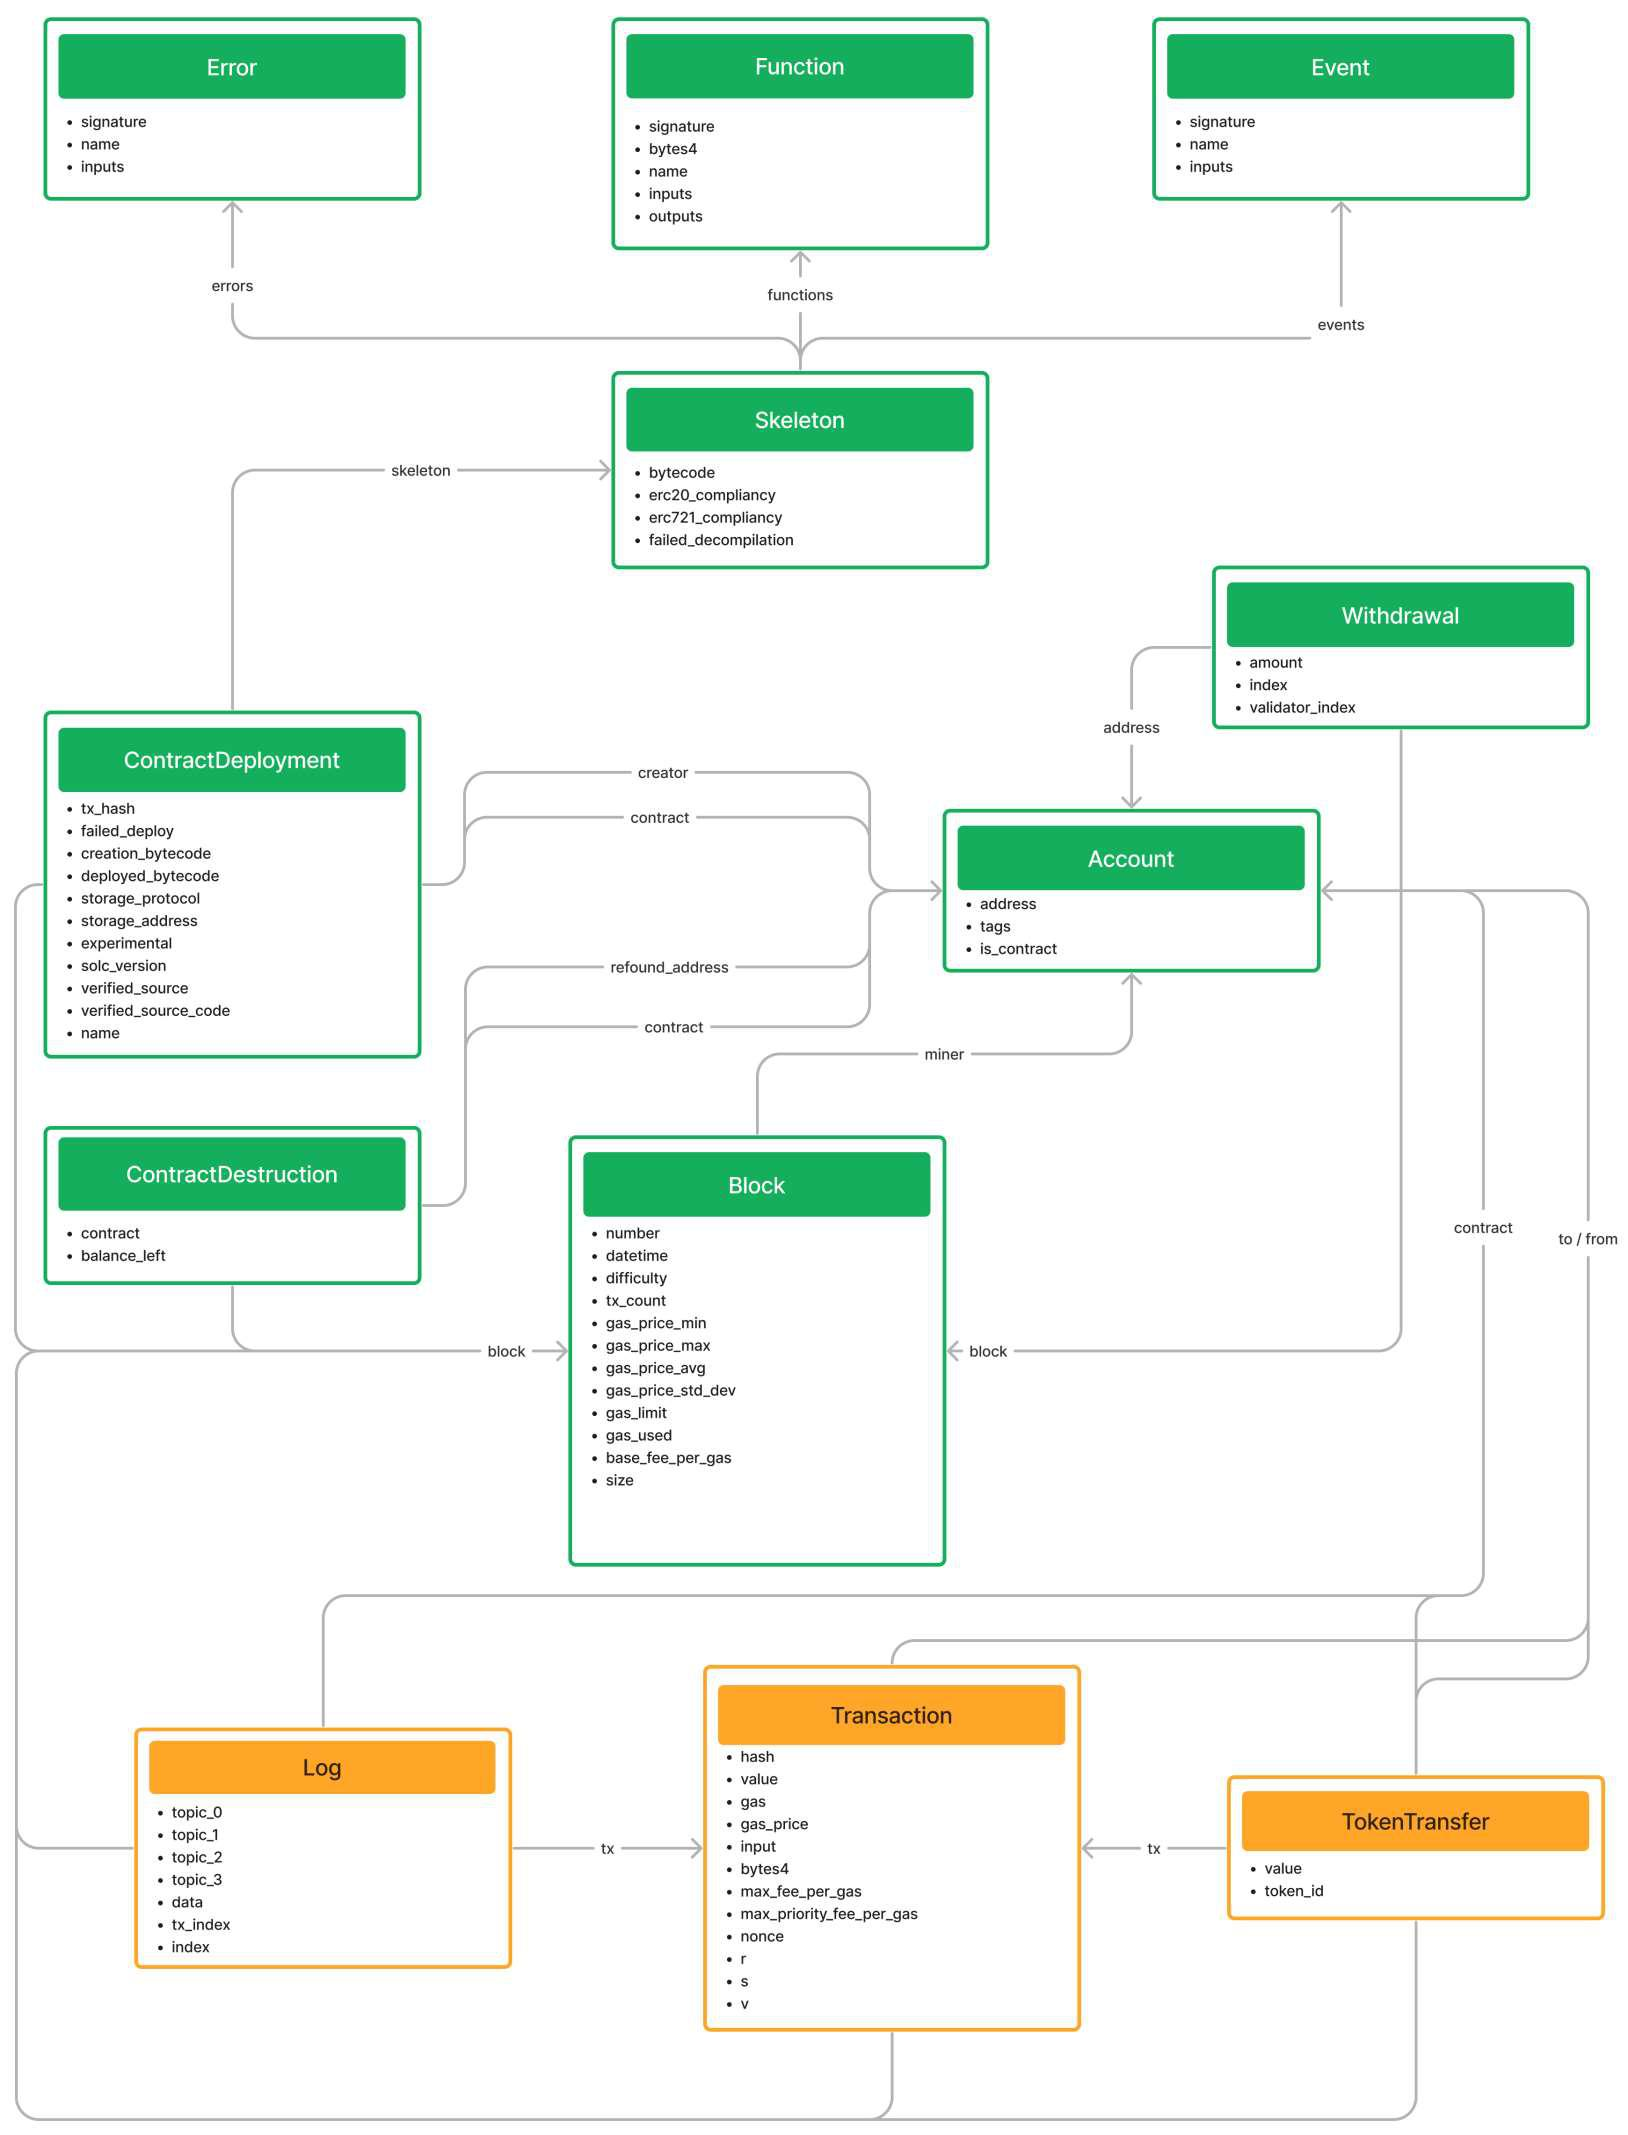
\includegraphics[width=0.7\textwidth]{resources/chapter-2/eth2dgraph-structure.jpg}
	\caption{Data model eth2dgraph \parencite{aimar2023extraction}}
	\label{image:eth2dgraph-structure}
\end{figure}

Penelitian yang dilakukan sebagai \textit{thesis} oleh \cite{aimar2023extraction} berfokus pada bagaimana mengambil data dari Blockchain Ethereum yang bersifat publik, mengekstrasi semantiknya, lalu mentransformasikannya ke sebuah bentuk yang mudah diakses oleh pengguna dengan cara mengindeksnya menggunakan Dgraph, sebuah \textit{open-source distributed graph database}. Hasil dari penelitian ini adalah sebuah perangkat lunak bernama eth2dgraph, yang ditulis dalam bahasa Rust yang melakukan mapping data Ethereum ke format Dgraph, dengan data model yang ditunjukkan pada gambar \ref{image:eth2dgraph-structure}. Perangkat lunak ini mengintegrasikan sebuah \textit{decompiler} untuk mengekstraksi dan mengindeks ABI dari Smart Contracts.

Salah satu fitur yang dapat dimanfaatkan dari riset ini adalah kemampuannya untuk mengekstrak data Smart Contracts dari Archive Node dengan efisien dan mengimpor data ke dalam format Dgraph. Selain itu, terdapat proses untuk menyambungkan data Smart Contract dengan \textit{source code} yang sesuai untuk Verified Smart Contracts yang didapatkan dari Smart Contract Sanctuary. 

Beberapa hal yang dapat diperhatikan dari perangkat lunak eth2dgraph adalah:

\begin{enumerate}
	\item Ekstraksi ABI \newline Cara eth2dgraph mengekstraksi semantik dari sebuah Smart Contract yang sudah dalam bentuk EVM Bytecode, yaitu dalam ABI (\textit{Application Binary Interface}). Gambar \ref{image:abi-extraction} menggambarkan bagaimana eth2dgraph memanfaatkan heimdall-rs untuk melakukan dekompilasi ABI. Cara ini dapat mengekstraksi lokasi fungsi, informasi terkait tipe \textit{input} dan \textit{output} dan nama fungsi, tetapi tidak memungkinkan untuk mengekstraksi nama parameter karena sudah dihilangkan pada saat kompilasi.
	      \begin{figure}[ht]
		      \centering
		      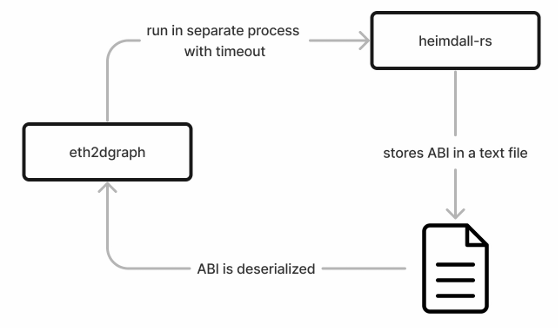
\includegraphics[width=0.7\textwidth]{resources/chapter-2/eth2dgraph-heimdall.png}
		      \caption{Ekstraksi ABI \parencite{aimar2023extraction}}
		      \label{image:abi-extraction}
	      \end{figure}
	\item Ekstraksi struktur dan metadata \newline Cara eth2dgraph mengekstraksi struktur Smart Contract dan metadata adalah menggunakan Regular Expression, dengan bagian \textit{runtime} diproses untuk mengekstraksi struktur, sedangkan bagian metadata dilakukan \textit{decode}.
	\item Ekstraksi menggunakan source code \newline eth2dgraph juga dapat melakukan ekstraksi semantik menggunakan source code yang tersedia dari sebuah Smart Contract, dengan cara melakukan query terhadap teks yang ada di dalam Smart Contract.
\end{enumerate}
